
\label{chapter:metodo}
Este Capítulo tem o objetivo de descrever a metodologia proposta neste trabalho, visando localizar e identificar objetos em ambientes confinados utilizando leitores e etiquetas passivas RFID, para gerenciamento e controle de bens.

\section{Visão geral do método}
O método consiste em um sistema que localiza qualquer objeto que tenha uma etiqueta RFID passiva fixada em seu corpo, as etiquetas serão localizadas e identificadas a medida em que transitam de uma sala para outra em um edifício. A localização e identificação é feita por meio de leitores RFID e controladores colados próximos a porta e os leitores devem ler tags que passam pela porta.
\par
Cada leitor junto ao controlador será responsável por uma sala, portanto qualquer etiqueta lida por aquele leitor ocasionará nas ações referentes a mesma sala. As ações poderá ser de atualização sobre a localização do objeto ou informando que o objeto está em transição para outra sala no edifício.
\begin{figure}[H]
              \caption{\label{fig:modelo}{Modelo Proposto}}
              \centering
              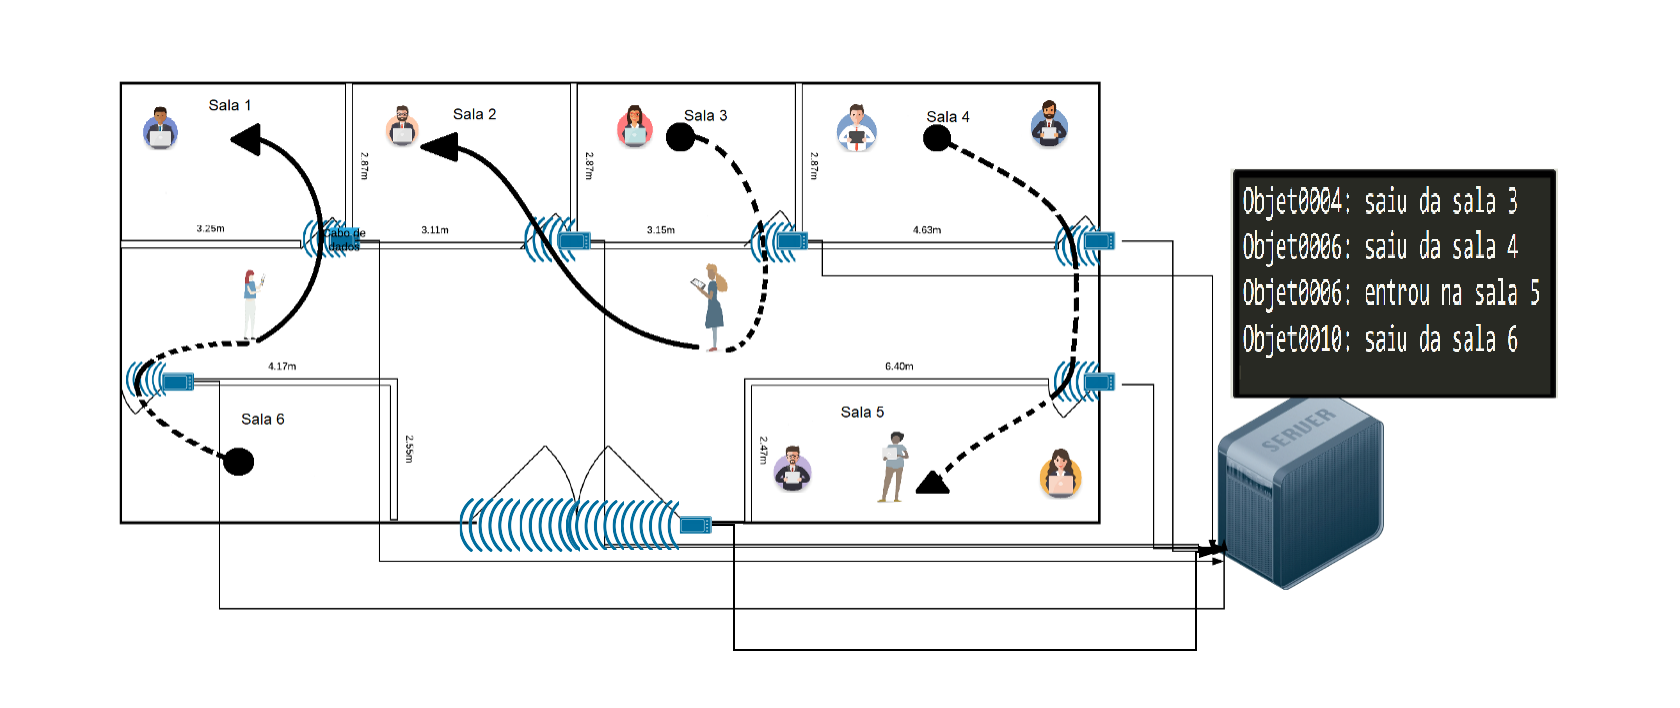
\includegraphics[width=1.1\textwidth]{Figuras/bigpicture.png}
              \legend{Fonte: Própria}
        \end{figure}
\par
Na \autoref{fig:modelo} é possivel notar que há um dispositivo acoplado proximo a porta de cada sala, esse dispositivo cotém o leitor RFID, esse dispositvo será encarrecado de consultar um servidor para assim tomar decisões do que será feito com o status do objeto, cada objtetos possui uma tag RFID fixada nele e quando passar pela porta o leitor identifica o objeto e altera sua as informações sobre sua localização.

\par
O método proposto consiste basicamente nas seguintes etapas:
\begin{enumerate}
    \item Identificação dos objetos rastreáves
    \item Monitoramento dos objetos rastreáves
    \item Localiazação do objetos em ambiente indoor
    \item Configuração do tempo para alertas
\end{enumerate}
\section{Identificação dos objetos rastreáveis}
Antes de qualquer passo é necessário a identificação dos objetos, nessa etapa é anexadas ao objetos as etiquetas RFID e realizada uma descrição do objeto portador dessa etiqueta no sistema, para que ao entrar e sair das salas do edificio além de fornecer a localização do objeto também seja possível ter detalhes sobre aquele objeto, dessa forma se objeto tiver uma registro local isso irá consta na descrição do objeto. Essa etapa pode ser considerada como a fase de cadastro.

\section{Monitoramento dos objetos rastreáveis}
O monitoramento é realizado pelos sensores RFID que estará em cada porta das salas do prédio e será responsável por enviar mensagens para o servidor sobre as ocorrências da sala para que medidas sejam realizadas.
\subsection{Fluxo de execução do método em cada sala}
Os dispositivos de cada sala terão o seguinte fluxo de execução apresentado na \autoref{fig:fluxograma}, o fluxo exemplifica as tarefas que cada dispositivos executarão. Neste fluxograma os retangulos represetam processos e retangulos com bordas duplas processos pré-deinidos, os losangos represetam as tomadas de decisões, os icones com bordas curvas para o mesmo lado represeta operações nos dados do sistema e o icone com bordas curvas oposta represeta o inicio do fluxo.
\begin{figure}[H]
              \caption{\label{fig:fluxograma}{Fluxograma de cada sala}}
              \centering
              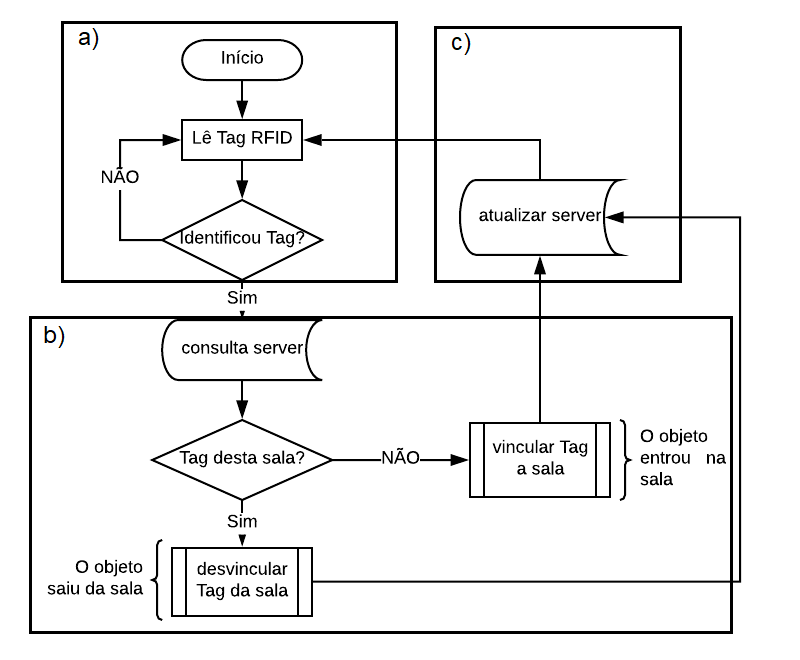
\includegraphics[width=1\textwidth]{Figuras/fluxograma.png}
              \legend{Fonte: Própria}
\end{figure}
\par
O fluxograma é separado em três modulos: \textbf{a}, \textbf{b} e \textbf{c}. O modulo \textbf{a} é onde é realizado o monitoramento da da sala, realizando leituras dos objetos que entram e saem da sala, no módulo \textbf{b} é o onde serão tomadas as decisões referente a etiqueta anexada ao objeto lida naquele momento, verificando se a etiqueta está ou não localizada naquela sala e processando as alterações necessárias. O módulo \textbf{c} é o último processo que atualiza as informações do servidor para que os dados consultados sejam iguais para todos. 
\section{Localização dos objetos}
Os objetos serão localizado no sistema baseado nos algoritmos de proximidade, ou seja, a partir do momento em que o leitor RFID identifica uma etiqueta, esse objeto terá a localização referente à aquele leitor, nesse sistema os leitores irão representar salas, portanto a localização indicará que o objeto estará na sala cujo o leitor que realizou a leitura representa.
\par
O sistema conterá um servidor que possui a função de tratar problemas relacionados a leituras de uma mesma etiqueta mais de uma vez, o papel do servidor é de grande importância também sendo utilizado para consultar informações referentes aos objetos.

\section{Configuração do tempo para alertas}

